\chapter{Описание экспериментов и результатов}

Глава посвящена проведенным экспериментам и их результатам.

\section{Предварительные эксперименты}

Для начала посмотрим на эксперименты, которые проводились до того, как тестировать все возможные версии моделей.

\subsection{Работа модуля генерации кандидатов}

Посмотрим на то, насколько хорошо работает модуль генерации кандидатов. При использовании модуля поиска на основе расстояния Дамерау-Левенштейна, максимальное расстояние было взято за единицу, ввиду резкого снижения производительности при увеличении данного значения. В таком случае, следует посмотреть насколько хорошо фонетическое кодирование и вручную заданные соответствия позволяют находить исправления на больших расстояниях. Результаты тестирования для ошибок вида <<один к одному>> см. в табл.~\ref{table:searher_results}.

\begin{table}[h]
	\begin{center}
		\caption{Работа модуля поиска кандидатов.}
		\label{table:searher_results}
		\begin{tabular}{|c|c|c|c|c|c|}
			\hline
			\textbf{Фон. код} & \textbf{Соотв.} & \textbf{РР} & \textbf{Кол. ошибок}  & \textbf{Кол. нахождений} & \textbf{Доля успехов}  \\
			\hline
			+ & - & \geq 2 & 341 & 110 & 31.3\% \\
			+ & - & 2 & 230 & 65 & 28.3\% \\
			+ & - & 3 & 75  & 28 & 37.3\% \\
			+ & - & 4 & 26  & 15 & 57.75\% \\
			+ & - & \geq 5 & 10 & 2 & 20\%  \\
			\hline
			- & + & \geq 2 & 341 & 99 & 29.0\% \\
			- & + & 2 & 230 & 54 & 23.5\% \\
			- & + & 3 & 75  & 31 & 41.3\% \\
			- & + & 4 & 26  & 7 & 26.9\% \\
			- & + & \geq 5 & 10 & 7 & 70\%  \\
			\hline
			+ & + & \geq 2 & 341 & 204 & 59.8\% \\
			+ & + & 2 & 230 & 115 & 50.0\% \\
			+ & + & 3 & 75  & 58 & 77.3\% \\
			+ & + & 4 & 26  & 22 & 84.6\% \\
			+ & + & \geq 5 & 10 & 9 & 90\%  \\
			\hline
		\end{tabular}
	\end{center}
\end{table}

Как видим, результаты работы двух рассматриваемых модулей практически не перескаются, т.е. один и тот же кандидат редко обнаруживается обоими модулями сразу. Всего удается находить около 60\% всех кандидатов на большом расстоянии Дамерау-Левенштейна, причем наибольшую трудность составляет расстояние, равное двум.

\subsection{Работа механизма объединения}

Аналогично, посмотрим насколько хорошо удается находить ошибки <<многие к одному>> при помощи механизма объединения последовательных токенов. Рассматривая только ошибки <<два к одному>> (ошибка другого типа была всего одна для обучающего датасета), получим:
\begin{itemize}
	\item количество ошибок: 69;
	\item количество срабатываний: 507;
	\item количество верных срабатываний (true positive): 40
	\item точность: 7.9\%;
	\item полнота: 58.0\%;
\end{itemize}

Как видим, доля ложных срабатываний очень велика. Посмотрим на примеры, когда такое происходит (в скобках выделены токены, на которых сработало объединение): 
\begin{itemize}
	\item \textit{В принципе, (я к) этому готова.}
	\item \textit{Провожаем жизнь (мы с) тобой.}
	\item \textit{Вы меня извините, (но я) опять про своих.}
\end{itemize}

Примеры демонстрируют, что токены могут объединяться совсем неподходящим образом.

Как было сказано при описании рассматриваемого механизма, была предпринята попытка объединения по расстоянию Дамерау-Левенштейна, но это лишь удвоило количество ложных срабатываний, почти не изменив TP.

\subsection{Обучение с учителем для модуля выбора позиции}

Как было описано в разделе про модель нахождения позиции, предпринималась попытка выбирать позиции не только на основе языковых моделей, но и при помощи других признаков.

Рассматриваемые признаки:
\begin{itemize}
	\item признаки позиции из модуля генерации кандидатов.
	\begin{itemize}
		\item индикатор написания с заглавной буквы;
		\item индикатор написания заглавными буквами;
		\item индикатор написания строчными буквами;
		\item индикатор первой позиции;
	\end{itemize}
	\item индикатор написания с заглавной буквы и не первой позиции;
	\item количество кандидатов;
	\item индикатор того, что текущий кандидат содержит дефис;
	\item признаки на основе вероятностей языковой модели для текущего кандидата:
	\begin{itemize}
		\item логарифм вероятности для текущего кандидата от языковой модели <<слева направо>>;
		\item логарифм вероятности для текущего кандидата от языковой модели <<справа налево>>;
		\item сагрегированное значение от языковых моделей для текущего кандидата.
	\end{itemize}
	\item признаки на основе источника кандидатов:
	\begin{itemize}
		\item доля кандидатов, пришедших из поиска, на основе Дамерау-Левенштейна;
		\item доля кандидатов, пришедших из поиска, на основе фонетического кодирования;
		\item доля кандидатов, пришедших из поиска, на основе вручную заданных соответствий;
	\end{itemize}
	\item признаки на основе доли более хороших кандидатов:
	\begin{itemize}
		\item доля кандидатов, лучше текущего, на основе языковой модели <<слева направо>>;
		\item доля кандидатов, лучше текущего, на основе языковой модели <<справа налево>>;
		\item доля кандидатов, лучше текущего, на основе сагрегированного показателя от обеих языковых моделей.
	\end{itemize}
	\item признаки на основе разницы между лучшим кандидатом и текущим:
	\begin{itemize}
		\item разница между лучшим кандидатом и текущим согласно языковой модели <<слева направо>>;
		\item разница между лучшим кандидатом и текущим согласно языковой модели <<справа налево>>;
		\item разница между лучшим кандидатом и текущим согласно сагрегированному показателю от обеих языковых моделей (признак, который использовался <<по-умолчанию>> до обучения с учителем).
	\end{itemize}
\end{itemize}

Решалась задача классификации позиции, как требующей исправления, выбиралась позиция с наибольшей предсказываемой вероятностью. В качестве метрики была выбрана обобщенная F-мера:

\begin{equation*}
	F_{\beta} = (1 + \beta^2) \frac{PR}{(\beta^2 P) + R},
\end{equation*}
где $P$ --- точность, $R$ --- полнота.

Было взято $\beta = 4$, чтобы отдать приоритет полноте, но при этом не классифицировать слишком много позиций, как требующие исправления.

Модель по-умолчанию --- это классификация позиции, как требующей исправления, на основе сравнения признака <<по-умолчанию>> с некоторым фиксированным значением $\alpha$. Посмотрим, как зависят различные метрики в зависимости от выбора $\alpha$, на рис.~\ref{ris:f4_plot_default}.

\begin{center}
	\begin{figure}[h!]
		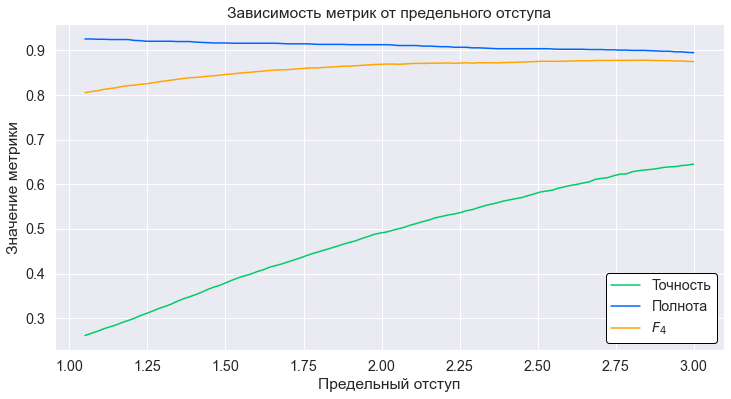
\includegraphics[width=\textwidth]{position_selector_default}
		\caption{График зависимости метрик от предельного отступа}
		\label{ris:f4_plot_default}
	\end{figure}
\end{center}

Итого, лучшее значение метрики достигаются при $\alpha = 2.84$. Аналогичным образом для сравнения была обучена  модель, игнорирующая исправления в заглавных позициях кроме первой. Затем были протестированы несколько моделей, учитывающих все признаки. Лучше всего показала себя логистическая регрессия с использованием взвешивания классов, реализованная в библиотеке scikit-learn. Посмотрим на все полученные результаты в табл.~ \ref{table:position_selector_comparison}.

\begin{table}[h]
	\begin{center}
		\caption{Сравнение версий модели выбора позиции исправления.}
		\label{table:position_selector_comparison}
		\begin{tabular}{|c|c|c|c|}
			\hline
			\textbf{Модель выбора позиции} & \textbf{Точность} & \textbf{Полнота} & $\boldsymbol{F_4}$  \\
			\hline
			По-умолчанию & 63.2\% & 90.0\%  & 87.8\% \\
			По-умолчанию + игнор. & 65.0\% & 89.8\%  & 87.8\% \\
			Лог. рег. & 73.7\% & 95.6\% & 94.0\%  \\
			\hline
		\end{tabular}
	\end{center}
\end{table}

Как видим, модель логистической регрессии, действительно, лучше, чем версия <<по-умолчанию>>. Она не только находит больше ошибок, но и имеет более хорошую точность. Проверим дает ли это прирост качества в применении к самой задаче. Для этого измерим качество модели исправления опечаток с отключенным механизмом объединения токенов и ранжирующей моделью SVM. Результаты см. в табл.~\ref{table:position_selector_extrinsic_comparison}

\begin{table}[h]
	\begin{center}
		\caption{Сравнение версий модели выбора позиции исправления в применении к исправлению опечаток.}
		\label{table:position_selector_extrinsic_comparison}
		\begin{tabular}{|c|c|c|c|}
			\hline
			\textbf{Модель выбора позиции} & \textbf{Точность}  & \textbf{Полнота} & $\boldsymbol{F_1}$  \\
			\hline
			По-умолчанию & 87.55 & 69.38 & 77.41 \\
			Лог. рег. & 87.48  & 68.27 & 76.69  \\
			\hline
		\end{tabular}
	\end{center}
\end{table}

Как видим, прироста в качестве нет, хотя прирост на задаче обучения был значительный. Объяснить это можно тем, что хоть модель и находит больше позиций с исправлениями, выполнить исправление не удается. Вполне возможно, что нет подходящих кандидатов. Например, модель понимает, что какое-то слово очень маловероятно согласно языковой модели, а потому там скорее всего опечатка, но подходящего кандидата на исправление нет. Модель <<по-умолчанию>> такой проблемой не обладает, так как выбирает только те позиции, для которых есть хорошее исправление.

\subsection{Эксперименты над моделью ранжирования}

Рассмотрим, как производилось измерение качества для моделей ранжирования. В частности, покажем, как выбиралась функция потерь для модели на основе CatBoost. 

Модели тестировались при помощи кросс-валидации по обучающим данным. В качестве целевой метрики была выбрана частота угадывания самого релевантного кандидата (такую метрику обычно обозначают как precision@1), так как по обучающим данным мы могли получить лишь одного правильного кандидата. Продемонстрируем результаты в табл.~\ref{table:catboost_losses_results}, полученные для случая, когда механизм объединения токенов был отключен.

\begin{table}[h]
	\begin{center}
		\caption{Сравнение различных функций потерь для модели ранжирования CatBoost.}
		\label{table:catboost_losses_results}
		\begin{tabular}{|c|c|}
			\hline
			\textbf{Модель ранжирования} & \textbf{Точность}  \\
			\hline
			- & 54.7\% \\
			SVM & 90.3\% \\
			CatBoost (\verb|RMSE|) & 91.9\% \\
			CatBoost (\verb|QueryRMSE|) & 92.1\% \\
			CatBoost (\verb|PairLogit|) & 92.7\% \\
			CatBoost (\verb|YetiRank|) & 92.4\% \\
			\hline
		\end{tabular}
	\end{center}
\end{table}

Отсутствие модели ранжирования означает, что берется модель исправления на основе BERT, то есть выбирается кандидат с самым большим средним логарифмом вероятностей для WordPiece-токенов.

Как видим, добавление дополнительных признаков вместе с ранжирующей моделью увеличивает качество очень значительно. В дальнейшем, при обсуждении модели CatBoost подразумевается, что используется функция потерь \verb|PairLogit|.

\section{Сравнение разных версий модели}

Посмотрим какие результаты демонстрируют различные версии моделей: см. табл.~\ref{table:versions_comparison}. Колонка <<BERT>> обозначает были ли использованы признаки BERT, колонка <<Объединение>> отвечает был ли использован механизм объединения смежных токенов. Используемые гиперпараметры:
\begin{itemize}
	\item версия BERT --- ConversationalRuBERT;
	\item версия языковой модели --- 3-граммная модель, обученная на всех данных;
	\item максимальное количество итераций --- 5;
	\item минимальный отступ при выборе лучшей позиции --- 2.5;
\end{itemize}

\begin{table}[h]
	\begin{center}
		\caption{Сравнение результатов вариаций модели.}
		\label{table:versions_comparison}
		\begin{tabular}{|c|c|c|c|c|c|}
			\hline
			\textbf{Ранжирование} & \textbf{BERT} & \textbf{Объединение} & \textbf{Точность}  & \textbf{Полнота} & $\boldsymbol{F_1}$  \\
			\hline
			- & + & - & 48.76 & 57.89 & 52.94 \\
			SVM & - & - & 86.52  & 67.26 & 75.68  \\
			SVM & - & + & 86.48  & 70.24 & 77.52  \\
			SVM & + & - & 87.55  & 69.38 & 77.41  \\
			SVM & + & +& 87.47 & 72.42 & 79.24 \\
			CatBoost & - & - & 86.14  & 67.00 & 75.38  \\
			CatBoost & - & + & 86.04  & 70.80 & 77.68  \\
			CatBoost & + & - & 87.34  & 69.13 & 77.18  \\
			CatBoost & + & + & \textbf{87.70} & \textbf{73.23} & \textbf{79.81} \\
			\hline
		\end{tabular}
	\end{center}
\end{table}

Как видим, использование других признаков вместе с ранжирующей функцией сильно улучшает качество. Существенный выигрыш в качестве получается как от добавления механизма объединения, так и от использования признаков BERT. В модели, использующей все улучшения, по-видимому, нет существенной разницы, что использовать для ранжирования: SVM или CatBoost.

\section{Эксперименты над гиперпараметрами лучшей версии модели}

Рассмотрим, как различные гиперпараметры влияют на качество лучшей модели. Исследуемые параметры:
\begin{itemize}
	\item Версия BERT:
	\begin{itemize}
		\item RuBERT;
		\item Conversational RuBERT.
	\end{itemize}
	\item Версия языковой модели:
	\begin{itemize}
		\item 3-граммная модель;
		\item 3-граммная модель без данных из социальных сетей;
		\item 4-граммная модель.
	\end{itemize}
	\item Максимальное число итераций.
	\item Минимальный зазор между лучшим и текущим кандидатами в модели выбора позиции.
\end{itemize}

Результаты тестирования отражены в табл.~\ref{table:hyperparam_results}. На первой строке указаны результаты модели по-умолчанию. Языковая модель с пометкой <<$3^*$>> обозначает версию 3-граммной модели, обученную без данных из социальных сетей. Как видим, прироста в качестве изменения гиперпараметров не дают.

\begin{table}[h]
	\begin{center}
		\caption{Сравнение результатов лучшей модели с различными гиперпараметрами.}
		\label{table:hyperparam_results}
		\begin{tabular}{|c|c|c|c|c|c|c|}
			\hline
			\textbf{BERT} & \textbf{ЯМ} & \textbf{Макс. ит.} & \textbf{Зазор} & \textbf{Точность} & \textbf{Полнота} & $\boldsymbol{F_1}$  \\
			\hline
			Conv. RuBERT & 3 & 5 & 2.5 & \textbf{87.70}  & 73.23 & \textbf{79.81} \\
			RuBERT & 3 & 5 & 2.5 & 87.01  & 72.22 & 78.93 \\
			Conv. RuBERT & 3 & 10 & 1.5 & 87.19  & \textbf{73.38} & 79.69 \\
			Conv. RuBERT & 4 & 5 & 2.5 & 86.86  & 72.57 & 79.07 \\
			Conv. RuBERT & $3^*$ & 5 & 2.5 & 86.99  & 70.70 & 78.00 \\
			\hline
		\end{tabular}
	\end{center}
\end{table}

\section{Сравнение с существующими решениями}

Посмотрим на то, как результаты лучшей модели соотносятся с уже существующими решениями: см. табл.~\ref{table:production_comparison}. Под быстрой моделью в таблице подразумевается лучшая модель, не использующая BERT. Данные взяты со страницы: \url{http://docs.deeppavlov.ai/en/master/features/models/spelling_correction.html} \cite{DeepPavlovTable}.  Как видим, даже быстрая версия оказывается лучше других решений.

\begin{table}[h]
	\begin{center}
		\caption{Сравнение результатов готовых моделей или сервисов.}
		\label{table:production_comparison}
		\begin{tabular}{|c|c|c|c|}
			\hline
			\textbf{Модель} & \textbf{Точность} & \textbf{Полнота} & $\boldsymbol{F_1}$  \\
			\hline
			Яндекс.Спеллер & 83.09  & 59.86 & 69.59 \\
			DeepPavlov & 59.38  & 53.44 & 56.25 \\
			SpellRuEval & 81.98  & 69.25 & 75.07 \\
			Лучшая версия & \textbf{87.70}  & \textbf{73.23} & \textbf{79.81} \\
			Быстрая версия & 87.55  & 69.38 & 77.41 \\
			\hline
		\end{tabular}
	\end{center}
\end{table}

\section{Недостатки модели}

Стоит отметить, что построенное решение имеет ряд недостатков:
\begin{enumerate}
	\item Низкая скорость работы. 
	
	На процессоре Intel Core i5-3210M, имеющем 2 ядра и 4 потока, версия, использующая BERT способна обрабатывать лишь около одного предложения за две секунды, что гораздо дольше, чем стандартные существующие решения. Около 80\% процессорного времени расходуется именно на BERT, а потому в быстрой версии скорость обработки удалось увеличить до примерно 4.5 предложений в секунду, что все равно достаточно мало. Тем не менее, возможно потенциальное ускорение с улучшением параллельной обработки предложений.
	
	\item Большое потребление памяти. 
	
	Модель потребляет порядка 7.5ГБ оперативной памяти. Большая часть уходит на хранение префиксного бора, позволяющего осуществлять поиск на заданном расстоянии Дамерау-Левенштейна. Тем не менее, стоит отметить, что имплементация этого модуля выполнена на языке Python, что открывает широкие возможности для оптимизации.
\end{enumerate}
